
\chapter{Fundamentação Teórica\label{chap:Fundamentacao}}

% Resumo opcional. Comentar se não usar.
%\resumodocapitulo{Resumo}

\section{Tecnologias comumente utilizadas}
 
 Existem diversos modos de estimar a ocupação de um certo ambiente por pessoas. Sensores de presença infravermelhos passivos já são amplamente utilizados comercialmente em aparelhos de ar-condicionado, especialmente modelos split para uso em pequenas salas.
 
 Sensores passivos de presença, entretanto, não permitem um controle mais fino da atuação do ar-condicionado. Eles auxiliam na economia de energia indicando a presença ou não de alguma pessoa ou animal no ambiente, mas sem indicar quantas pessoas etão no local ou quais são suas características. Além disso estão muito sujeitos a interferências, causando falsos positivos ou falsos negativos, devido ao modo de atuação passivo que apenas verifica a emissão de radiação infravermelha em comprimentos de onda próximos ao dos humanos.

 Uma alternativa possível é o uso de RFID. Esta é uma tecnologia que torna-se mais eficiente, acessível e popular a cada dia. O monitoramento posicional de objetos dentro de uma loja ou armazém tornou-se uma prática possível com RFID passivo, prática que é aplicada com soluções comerciais disponíveis no mercado.
 
\section{RFID}

A comunicação do tipo Identificação por Radiofrequência – \textit{Radio Frequency Identification} (RFID) – é um tipo de comunicação sem fio por sinais de rádio. O RFID é uma alternativa de identificação útil em aplicações que exigem a leitura de grandes quantidades de dados \cite{rao1999overview}. 

A composição geral do RFID é feita por uma \textit{TAG} ou etiqueta e uma leitora (reader) que são incorporadas com um transmissor e um receptor no computador \cite{EPC-RFID-link}.

\begin{figure}[H]
    \centering
    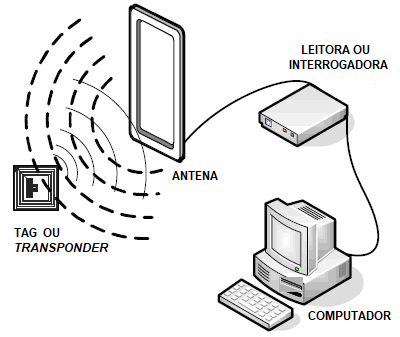
\includegraphics[width=0.6\linewidth]{figs/Fundamentos/Composicao.png}
    \caption{\textcolor{red}{Composição básica de um sistema RFID. (Fonte: EPC-RFID...)}}
    \label{fig:ComposicaoRFID}
\end{figure}


As primeiras aplicações comerciais de RFID, como artigo eletrônico de vigilância (Electronic Article Surveillance), aconteceram no final da década de 1960, desenvolvidas por empresas como: Kongo, Sensormatic (by Johnson Controls) e Checkpoint \cite{chawla2007overview}.

De acordo com Chawla e Ha \cite{chawla2007overview}, o sistema RFID consiste em leitoras e TAGS. A leitora tem como função se comunicar na faixa de alcance sem fio e coletar informações sobre os objetos aos quais as TAGS estão anexadas (ex.: entrada e saída de pessoas de um estabelecimento).

\begin{figure}[H]
    \centering
    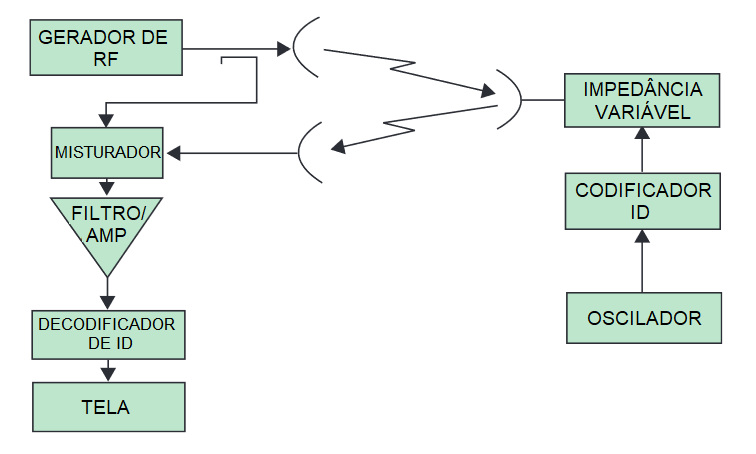
\includegraphics[width=0.6\linewidth]{figs/Fundamentos/RFIDdiagram.png}
    \caption{Diagrama de rede de uma comunicação RFID. (Adaptado de Landt, Jeremy \cite{landt2005history}}
    \label{fig:DiagramaRFID}
\end{figure}

\begin{figure}[H]
    \centering
    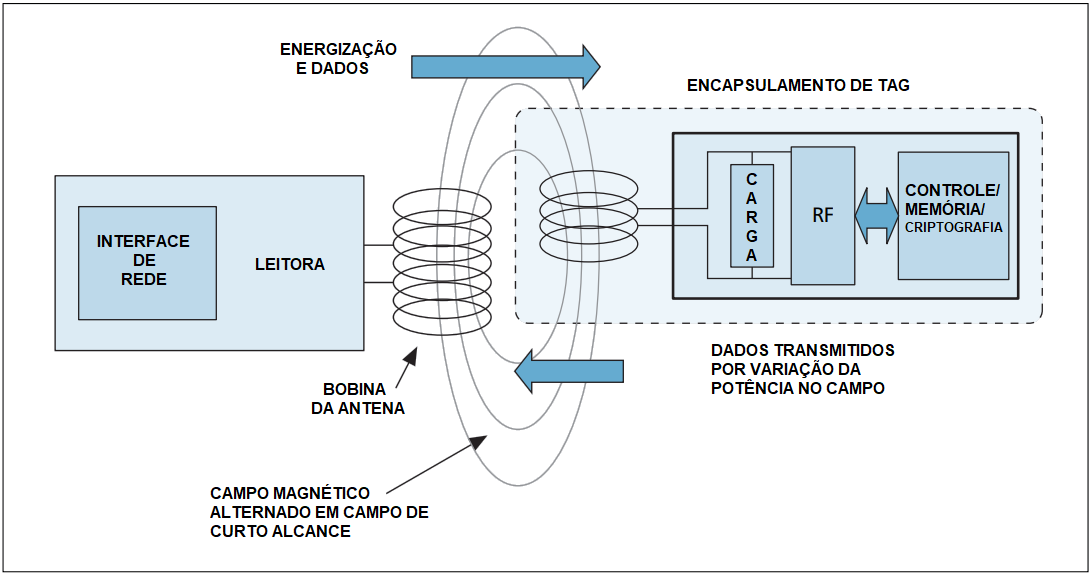
\includegraphics[width=0.8\linewidth]{figs/Fundamentos/RFIDdetails.png}
    \caption{\textcolor{red}{Composição básica de um sistema RFID. (Chawla e Ha, 2007)}}
    \label{fig:DetalhesRFID}
\end{figure}



Vogt \cite{vogt2002multiple}, em seu trabalho, investigou a aplicabilidade da RFID passiva na identificação de múltiplos objetos.

\begin{figure}[H]
    \centering
    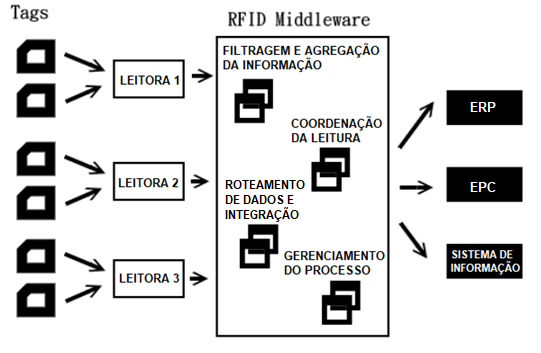
\includegraphics[width=0.6\linewidth]{figs/Fundamentos/RFID.png}
    \caption{\textcolor{red}{RFID - . (Fonte: Adaptado de Chen et al., 2008) }}
    \label{fig:AntenaThresholdCoverage}
\end{figure}


\subsection{RAIN RFID}

O padrão RAIN (acrônimo para \textit{RAdio frequency IdentificatioN} - Identificação por radiofrequência) é a união de diferentes tipos de hardware e software que possuem o propósito de ligar o meio RFID UHF com a computação em nuvem. É padronizada pela organização global de mesmo nome (RAIN) com o objetivo de popularizar o uso de RFID. \cite{RAIN}

\subsection{\textit{TAGs}}
TAGs, também conhecidas como transponders, são etiquetas ou chips microprocessadores de identificação. Esses dispositivos recebem sinal de rádio e transmitem, automaticamente, um sinal diferente. Cada TAG possui um número serial de identificação que a difere de outras. \cite{chawla2007overview}. Esses objetos podem armazenar informações como \textit{serial number} (número serial), \textit{model number} (número do modelo), bem como outras características como: data, cor, tamanho e preço. A TAG RFID é classificada de acordo com sua memória, tipo de comunicação e uso de energia, como é possível visualizar na tabela \textcolor{red}{NUMERO DA TABELA}.  \cite{AhmedIntegrationStreamMapping}.


\huge \textcolor{red}{[Tabela]} \normalsize

É possível classificar as TAGs em três tipos, como pode ser visto na tabela \textcolor{red}{NUMERO DA TABELA}: ativas, passivas e semi-passivas \cite{chawla2007overview}.  Existem vários tipos de TAGS ativas (alimentadas por baterias) e passivas, em várias faixas de frequência, presentes no mercado \cite{rao1999overview}. A Figura \textcolor{red}{NUMERO DA FIGURA}, logo abaixo, mostra exemplos de TAGS ativas e passivas.

Segundo Rao \cite{rao1999overview}, TAGS ativas, como as apresentadas na Figura 1A, tem como vantagens o fornecimento de faixas de leituras maiores (explicar o porquê isso é interessante). Como desvantagem, elas podem ser bem mais caras por exigirem o uso de baterias \cite{rao1999overview}. Uma etiqueta RFID passiva, por sua vez, usará a energia das ondas de rádio do interrogador para retransmitir suas informações armazenadas de volta ao interrogador \cite{EPC-RFID-link}. 

\subsection{Antenas}

A antena é capaz de perceber o sinal de uma TAG dentro de um determinado raio de cobertura. Cada antena é única nesse sentido...